
%%% Local Variables:
%%% mode: latex
%%% TeX-master: t
%%% End:

\documentclass{beamer}

\usetheme{boxes}
\usepackage[utf8]{inputenc}
\usepackage{tikz}
\usetikzlibrary{calc,shapes.multipart,chains,arrows}

\begin{document}

\begin{frame}

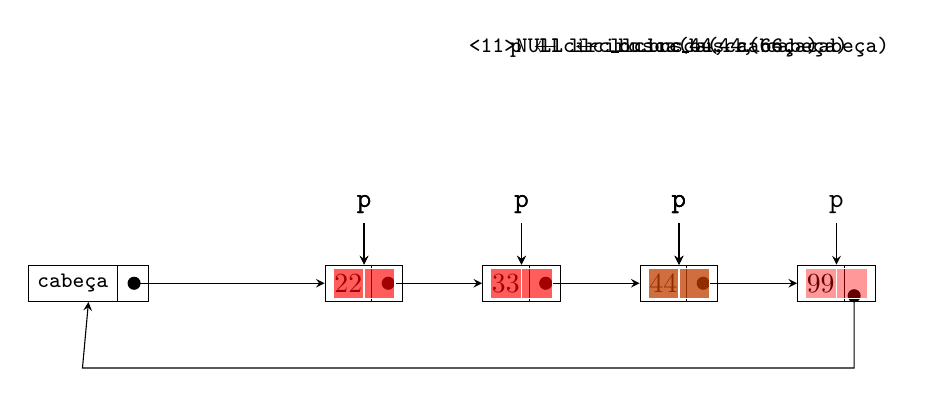
\begin{tikzpicture}
\def\shift{2cm}
\def\cabeca{{\tt cabe\c{c}a}}

\tikzset{
    list/.style={rectangle split, rectangle split parts=2,
    draw, rectangle split horizontal}, 
    >=stealth, start chain
}

  \node[list,on chain] (HEAD) {\footnotesize \cabeca};
  \node[] (BACKLINK) [below of=HEAD] {};

  \node[]  (FIRST) [right of=HEAD,xshift=.5*\shift]  {};
  \node[]  (SECOND) [right of=FIRST,xshift=.5*\shift] {};
  \node[]  (THIRD) [right of=SECOND,xshift=.5*\shift] {};
  \node[]  (FOURTH) [right of=THIRD,xshift=.5*\shift] {};
  \node<1->[list,on chain] (C) at (FIRST) {22};
  \node<1->[list,on chain] (A) at  (SECOND) {33};
  \node<1->[list,on chain]  (B) at (FOURTH) {99};
  \node<1->[list,on chain]  (D) at (THIRD) {44};
  
  %BUSCA 44
   \def\tail{D}
   \node<1-4> [above of=\tail,yshift=\shift] {{\tt\footnotesize llcirc\_busca(44, \cabeca)}};
   \draw<1->[*->] let \p1 = (HEAD.two), \p2 = (HEAD.center) in (\x1,\y2)  -- (C);
   \draw<1->[*->] let \p1 = (C.two), \p2 = (C.center) in (\x1,\y2) -- (A);
   \draw<1->[*->] let \p1 = (A.two), \p2 = (A.center) in (\x1,\y2) -- (D);
   \draw<1->[*->] let \p1 = (D.two), \p2 = (D.center) in (\x1,\y2)  -- (B);
   \draw<1->[*->] (B.two) -- +(0,-.5*\shift) --
   +(-4.9*\shift,-.5*\shift) -- (HEAD.south);

   % POINTER
   \foreach \s/\l in {2/C, 3/A, 4/D} {
     \node<\s>  (p\s) [above of=\l] {\tt p};
     \path<\s>[->,draw] (p\s) -- (\l);
     \node<\s>[white,list,fill=red, fill opacity=.4] at (\l) {};
    }
    % FOUND
     \node<5> [above of=\tail,yshift=\shift] {{\tt\footnotesize p $\leftarrow$ llcirc\_busca(44, \cabeca)}};
     \node<5>  (p5) [above of=D] {\tt p};
     \path<5>[->,draw] (p5) -- (D);
     \node<5>[white, list, fill=green, fill opacity=.3] at (D) {};

   % POINTER
   \node<6-11> [above of=\tail,yshift=\shift] {{\tt\footnotesize \onslide<11>{NULL $\leftarrow$} llcirc\_busca(66, \cabeca)}};
   \foreach \s/\l in {7/C, 8/A, 9/D, 10/B} {
     \node<\s>  (p\s) [above of=\l] {\tt p};
     \path<\s>[->,draw] (p\s) -- (\l);
     \node<\s>[white,list,fill=red, fill opacity=.4] at (\l) {};
    }
   

    

\end{tikzpicture}

\end{frame}

\end{document}